%% Intro
In this chapter we want to figure out the effect of different parameters on the response time and the throughput with a 2k analysis. \\
More specifically, we conduct a $2^k*r$ analysis with three factors ($k=3$) and with three repetitions ($r=3$). The analysis is done for two different workloads (read-only and write-only) and for two different response variables (throughput and response time), i.e. in total we conduct four $2^k*r$ analyses. \\
The three factors we consider are the number of memcached servers, the number of middlewares and the number of worker threads. Each factor can assume two levels ($-1$ and $1$), which represent a specific configuration as given in the following table:
\begin{center}
	\scriptsize{	
		\begin{table}[!ht]
			\centering
			\begin{tabulary}{\linewidth}{ | C | C | C | C | }
				\hline 	&	Number of servers (\textbf{A})	&	Number of middlewares (\textbf{B})	& Number of workers (\textbf{C})	\\
				\hline	-1	&	1	&	1	&	8	\\
				\hline	1	&	3	&	2	&	32	\\
				\hline 
			\end{tabulary}
		\end{table}
	}
\end{center}
To get the input data of the analysis we first need to run the experiments. We let each experiment run for 90s and each experiment is repeated 3 times.  The first and last 10 seconds of an experiment are part of the warm-up and cool-down phase and are thus ignored. The overview of the experiment parameters is shown in the following table:
\begin{center}
	\scriptsize{
		\begin{tabular}{|l|c|}
			\hline Number of servers                & 1 and 3                                     \\ 
			\hline Number of client machines        & 3                                           \\ 
			\hline Instances of memtier per machine & 1 (1 middleware) or 2 (2 middlewares) \\ 
			\hline Threads per memtier instance     & 2 (1 middleware) or 1 (2 middlewares)   \\
			\hline Virtual clients per thread       &  32                                     \\ 
			\hline Workload                         & Write-only and Read-only\\
			\hline Number of middlewares            & 1 and 2                                     \\
			\hline Worker threads per middleware    & 8 and 32                                    \\
			\hline Repetitions                      & 3                                  \\ 
			\hline 
		\end{tabular}
	} 
\end{center}

% additive or multiplicative model
The multiplicative model was chosen for all four analyses. It assumes that the effect of the factors, their interactions and the errors are multiplicative. The multiplicative model does explain our data very well because the unexplained variation of effects is less than $0.65\%$ in all analyses.
All we have to do in the multiplicative model in contrast to the additive one, is to take the log of the measurements. Then the calculations remain the same.  \\

% explain tables
Before doing the interpretation of the results of the analyses, we want to explain what has been done in the tables which can be found at the end of this section. Note that all computations are done as explained in chapter $18$ of the book "The Art of Computer Systems Performance Analysis" by Raj Jain\footnote{Raj Jain, The Art of Computer Systems Performance Analysis: Techniques for Experimental Design, Measurement, Simulation, and Modeling, April 1991, ISBN: 978-0471503361.}. 
First of all, the input data, which is the measured response for different configurations and repetitions, is colored in yellow. Note that we take the log because of the multiplicative model. 
The effect variables $q$ can be computed using the sign table method. The signs of the sign table are colored in red, while the effect variables are colored in green. The importance of a factor $j$ is computed as the proportion of total variance in the response that is explained by that factor. It can be computed as $SSj/SST$, where $SST$ (the Sum of Squares Total) is the total variance of the response $y$ and $SSj$ (the Sum of Squares due to factor $j$) is the portion of $SST$ that is explained by factor $j$.
The difference between the estimated and measured response values are called the experimental errors and are colored in purple. The Sum of Squared Errors (SSE) is used to estimate the variance of the errors and to compute the confidence intervals for the effects for which the t-value at $16$ ($=2^k(r-1)$) degrees of freedom and $90\%$ confidence was chosen. If $0$ is included in the confidence interval, the effect can be considered insignificant. \\


%% write only
$\bullet$ \textbf{Write-only workload:} The number of middlewares explains $73.5\%$ of the variation of effects on the throughput, which is by far the strongest effect. Then we have the number of servers with $14.7\%$ of variation of effects on the throughput but they have a negative effect. The number of workers have $7.9\%$ variation of effects on the throughput and a positive effect. \\
Those numbers make sense: In section \ref{section:BaselineWithMW} we saw that for the write-only workload going from 1 to 2 middlewares almost doubled the maximum achievable throughput because the net-thread bottleneck was relieved. Increasing the workers also increased the throughput because more requests can be processed in parallel, but not as significant as going from 1 to 2 middlewares. Increasing the number of servers has a negative effect on the throughput because of the replication that adds overhead to the system. \\
Almost all interactions-effects are either statistically insignificant or can be considered negligible, with the exception of the interaction-effect of the middlewares and the workers, which has $2.5\%$ of variation of effects. This is because increasing the number of middlewares also increases the number of workers. \\
The percentages of variation of throughput and response time are basically the same with small deviations, which is what we expect because of the interactive response time law. But for the response time, the sign of significant effects are opposite to the throughput because they relate inverse proportionally to each other. \\

%% read-only
$\bullet$ \textbf{Read-only workload:} For the read-only workload the variation of effects can be explained entirely by the number of servers. All other effects are statistically insignificant or negligible. \\
This is because of the outbound network bandwidth bottleneck at the servers. If we fix the number of servers, this bottleneck puts a hard limit on the maximum achievable throughput, which we can also compute as  (maximum bandwidth per server * \#servers)/ size of a Get response. Thus changing number of workers (8 or 32) or changing the number of middlewares (1 or 2) does not change anything regarding throughput under this bottleneck. But going from 1 to 3 servers increases throughput from 3k ops/s to almost 9k ops/s because we have three times more outbound network bandwidth at the servers in total. \\
The response time analysis also conforms to the throughput analysis and relates in the same way to it as explained for the write-only workload. 

%% insert tables
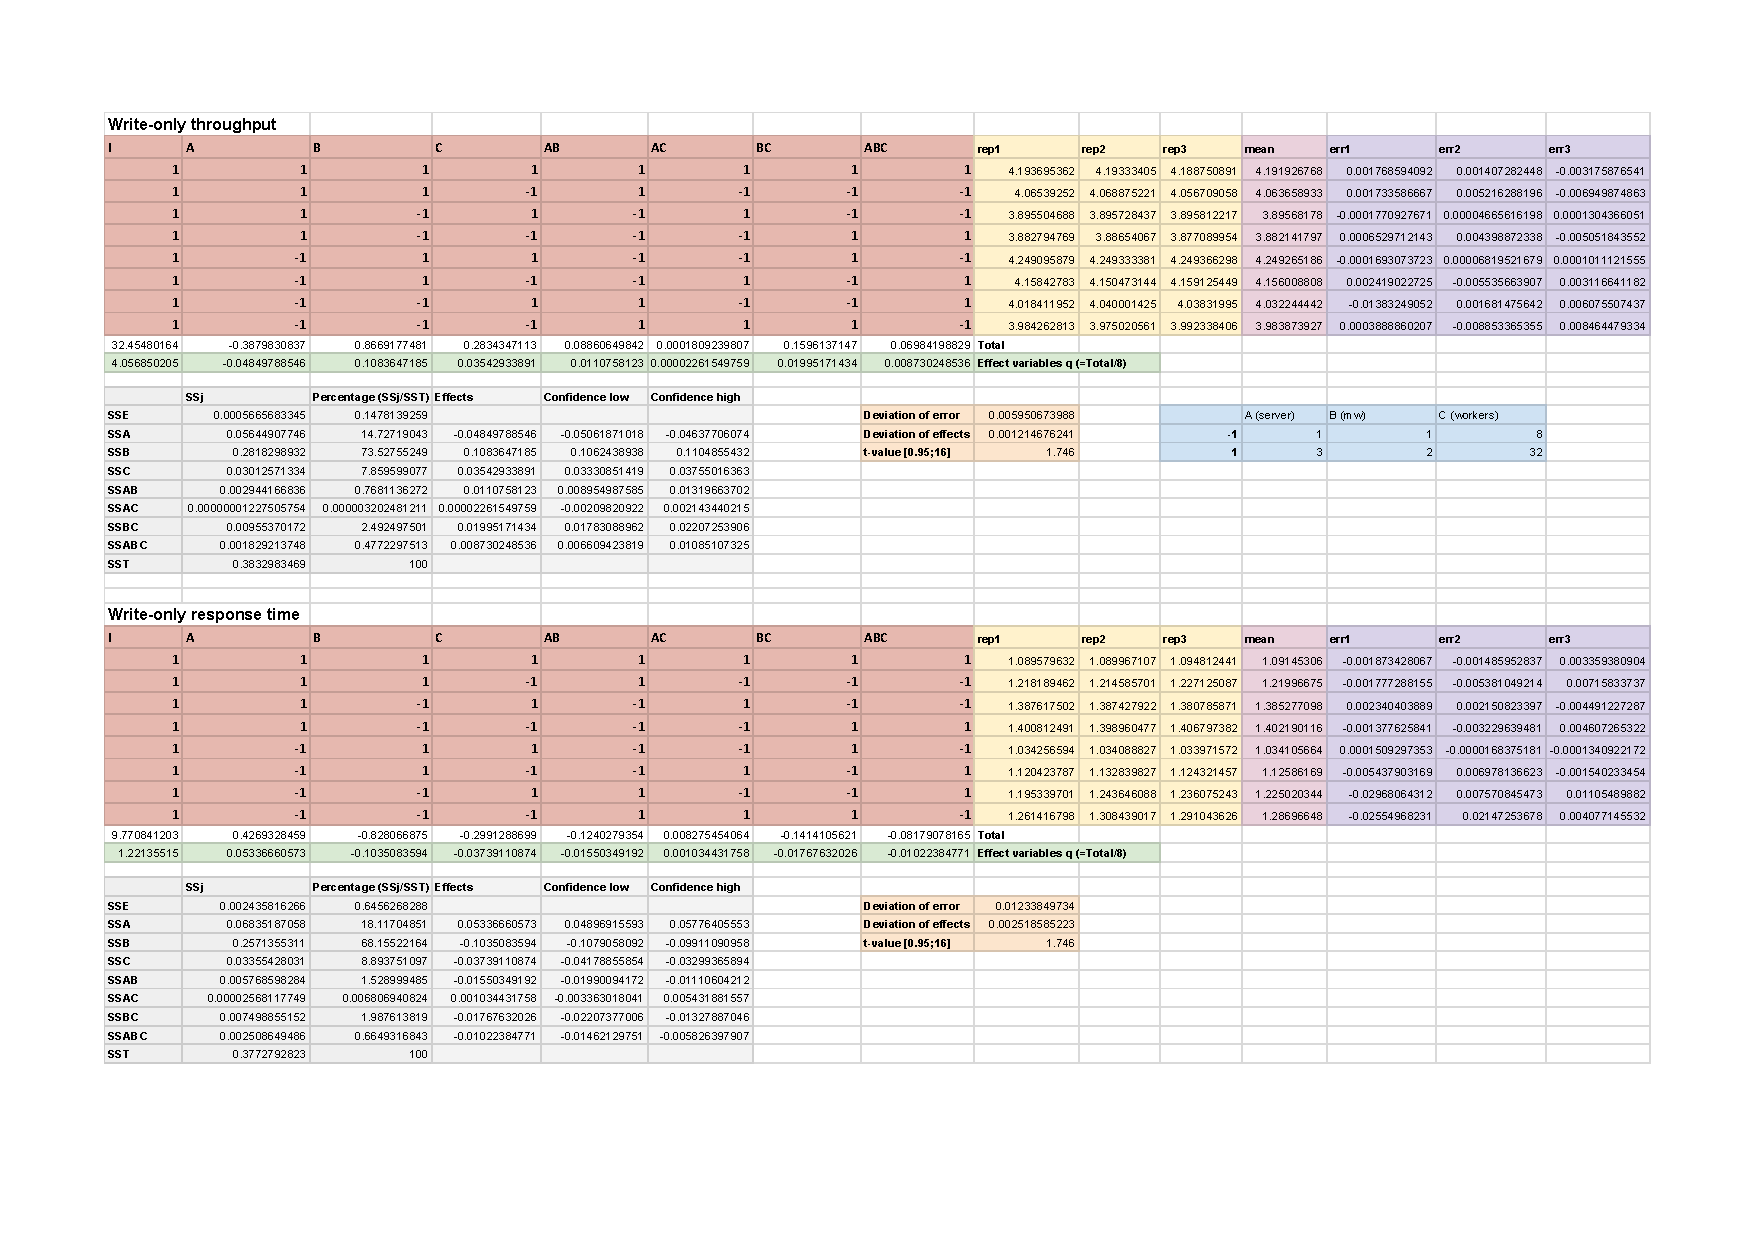
\includepdf[pages=-,scale=1,landscape=true]{figures/5_2kAnalysis/2kAnalysis_multiplicative_WO_2018-11-15_07h37.pdf}
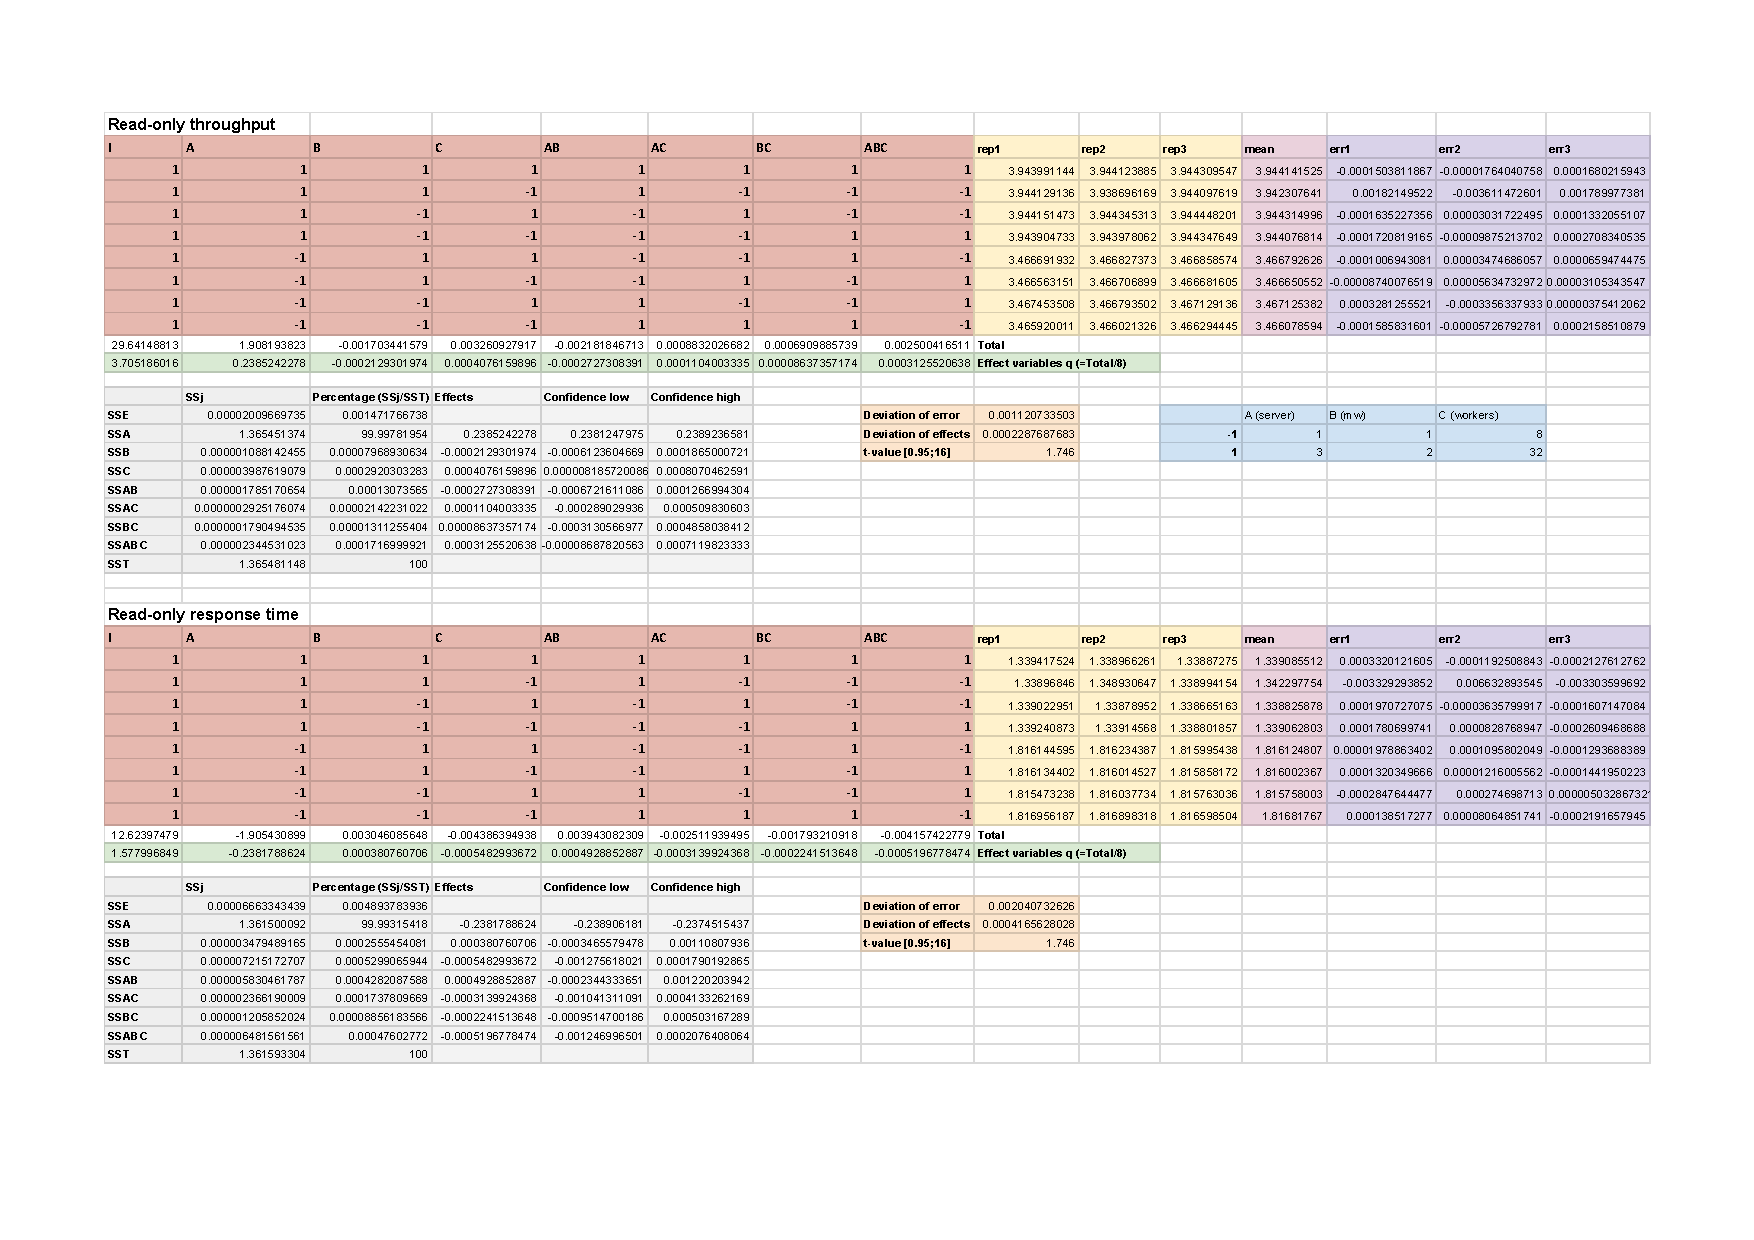
\includepdf[pages=-,scale=1,landscape=true]{figures/5_2kAnalysis/2kAnalysis_multiplicative_RO_2018-11-15_07h37.pdf}